\documentclass{book}
\usepackage{amssymb,amsmath}
\usepackage{polyglossia}
\setmainlanguage{spanish} % Idioma principal
\usepackage{theorem}
\usepackage{times}
\usepackage{array}
\usepackage{graphicx}
\usepackage{hyperref}
\usepackage{multirow}
\usepackage{fancyhdr}
%\usepackage[cp1252]{inputenc}
\usepackage{hhline}
\usepackage{multicol}
\usepackage[a4paper,driver=xetex,top=4.5cm,head=4.5cm, bottom=2cm,%
layouthoffset=0mm, left=2.5cm, right=2.5cm,marginparwidth=0cm]{geometry}
%\usepackage{bm}
%\usepackage{tabular}
\usepackage{fontspec}
 \usepackage[breakable,many]{tcolorbox}
\defaultfontfeatures{Ligatures=TeX}
\usepackage{empheq}
 \setromanfont{Roboto Condensed}
 \usepackage{float}
 \usepackage{mathrsfs} 
%
%
% \renewcommand{\familydefault}{\sfdefault}
%\renewcommand{\familydefault}{\sfdefault}

%%%%%%%%%Estilo de la pagina%%%%%%%%%%%%%%%%%%%%%%%%%%%%%%%%%%%
%%%%%%%%%%%%%%%%%%%%%%%%%%%%%%%%%%%%%%%%%%%%%%%%%%%%%%%%%%%%%%%%%%
% \newcounter{ejer}
% 
% {\theorembodyfont{\normalfont}
% \newtheorem{ejercicio}[ejer]{Ejercicio}}

\newcommand{\rr}{\mathbb{R}}
\newcommand{\qq}{\mathbb{Q}}
\newcommand{\nn}{\mathbb{N}}



\DeclareMathOperator{\atan2}{atan2}
%\DeclareMathOperator{\sen}{sen}
\DeclareMathOperator{\sign}{sign}
\DeclareMathOperator{\sn}{sn}
\DeclareMathOperator{\SO}{SO}
%\DeclareMathOperator{\arcsen}{arcsen}
\DeclareMathOperator{\Or}{O}

\usepackage[framemethod=TikZ]{mdframed}
%%%%%%%%%%%%%%%%%%%%%%%%%%%%%%
%Theorem

%% Ejercicio
\newcounter{ejer} \setcounter{ejer}{0}
\renewcommand{\theejer}{\arabic{ejer}}
\newenvironment{ejer}[2][]{%
\vspace{5pt}
\refstepcounter{ejer}%
\ifstrempty{#1}%
{%
% \mdfsetup{%
% frametitle={%
% \tikz[baseline=(current bounding box.east),outer sep=-0pt]
% \node[anchor=east,rectangle,fill=green!50]
{\noindent\bfseries Ejercicio~\theejer}.}
%
{%
% \mdfsetup{%
% frametitle={%
% \tikz[baseline=(current bounding box.east),outer sep=0pt]
% \node[anchor=east,rectangle,fill=green!50]
{\noindent\bfseries  Ejercicio~\theejer:~#1};}%
%
%\mdfsetup{innertopmargin=10pt,linecolor=green!50,%
%linewidth=2pt,topline=true,%
%frametitleaboveskip=\dimexpr-\ht\strutbox\relax
%}
%\begin{mdframed}[]
\relax%
\label{#2}}{\vspace{5pt}}%\end{mdframed}}

%Theorem
\newcounter{theo}[chapter] \setcounter{theo}{0}
\renewcommand{\thetheo}{\arabic{section}.\arabic{theo}}
\newenvironment{theo}[2][]{%
\refstepcounter{theo}%
\ifstrempty{#1}%
{\mdfsetup{%
frametitle={%
\tikz[baseline=(current bounding box.east),outer sep=0pt]
\node[anchor=east,rectangle,fill=blue!20]
{\strut Teorema~\thetheo};}}
}%
{\mdfsetup{%
frametitle={%
\tikz[baseline=(current bounding box.east),outer sep=0pt]
\node[anchor=east,rectangle,fill=blue!20]
{\strut Teorema~\thetheo:~#1};}}%
}%
\mdfsetup{innertopmargin=10pt,linecolor=blue!20,%
linewidth=2pt,topline=true,%
frametitleaboveskip=\dimexpr-\ht\strutbox\relax
}
\begin{mdframed}[]\relax%
\label{#2}}{\end{mdframed}}
%%%%%%%%%%%%%%%%%%%%%%%%%%%%%%
%Lemma
\newcounter{lem}[chapter] \setcounter{lem}{0}
\renewcommand{\thelem}{\arabic{section}.\arabic{lem}}
\newenvironment{lem}[2][]{%
\refstepcounter{lem}%
\ifstrempty{#1}%
{\mdfsetup{%
frametitle={%
\tikz[baseline=(current bounding box.east),outer sep=0pt]
\node[anchor=east,rectangle,fill=green!20]
{\strut Lemma~\thelem};}}
}%
{\mdfsetup{%
frametitle={%
\tikz[baseline=(current bounding box.east),outer sep=0pt]
\node[anchor=east,rectangle,fill=green!20]
{\strut Lemma~\thelem:~#1};}}%
}%
\mdfsetup{innertopmargin=10pt,linecolor=green!20,%
linewidth=2pt,topline=true,%
frametitleaboveskip=\dimexpr-\ht\strutbox\relax
}
\begin{mdframed}[]\relax%
\label{#2}}{\end{mdframed}}
%%%%%%%%%%%%%%%%%%%%%%%%%%%%%%
%% Definicion
\newcounter{defini}[chapter] \setcounter{defini}{1}
\renewcommand{\thedefini}{\arabic{section}.\arabic{defini}}
\newenvironment{definicion}[2][]{%
\refstepcounter{defini}%
\ifstrempty{#1}%
{\mdfsetup{%
frametitle={%
\tikz[baseline=(current bounding box.east),outer sep=0pt]
\node[anchor=east,rectangle,fill=green!20]
{\strut Definición~\thedefini};}}
}%
{\mdfsetup{%
frametitle={%
\tikz[baseline=(current bounding box.east),outer sep=0pt]
\node[anchor=east,rectangle,fill=green!20]
{\strut Definición~\thedefini:~#1};}}%
}%
\mdfsetup{innertopmargin=10pt,linecolor=green!20,%
linewidth=2pt,topline=true,%
frametitleaboveskip=\dimexpr-\ht\strutbox\relax
}
\begin{mdframed}[]\relax%
\label{#2}}{\end{mdframed}}

%Proof
\newenvironment{prf}{\noindent\emph{Dem.}}{$\square$ \newline\vspace{5pt}}


%Corolario
\newcounter{cor}[chapter] \setcounter{cor}{0}
\renewcommand{\thecor}{\arabic{section}.\arabic{cor}}
\newenvironment{cor}[2][]{%
\refstepcounter{cor}%
\ifstrempty{#1}%
{\mdfsetup{%
frametitle={%
\tikz[baseline=(current bounding box.east),outer sep=0pt]
\node[anchor=east,rectangle,fill=green!20]
{\strut Corolario~\thelem};}}
}%
{\mdfsetup{%
frametitle={%
\tikz[baseline=(current bounding box.east),outer sep=0pt]
\node[anchor=east,rectangle,fill=green!20]
{\strut Corolario~\thelem:~#1};}}%
}%
\mdfsetup{innertopmargin=10pt,linecolor=green!20,%
linewidth=2pt,topline=true,%
frametitleaboveskip=\dimexpr-\ht\strutbox\relax
}
\begin{mdframed}[]\relax%
\label{#2}}{\end{mdframed}}

\tcbset{highlight math style={enhanced,
  colframe=red!60!black,colback=yellow!50!white,arc=4pt,boxrule=1pt,
  drop fuzzy shadow}}
  
  
  
  
  
  
  


\pagestyle{fancyplain}

 \renewcommand{\sectionmark}[1]
                 {\markright{\thesection\ #1}}


% \lhead[\fancyplain{}{\bfseries\thepage}]
%       {\fancyplain{}{\bfseries\rightmark}}
%
 \rhead[\fancyplain{}{\bfseries\leftmark}]{\fancyplain{}{\bfseries}}




 \lhead[\fancyplain{}{ 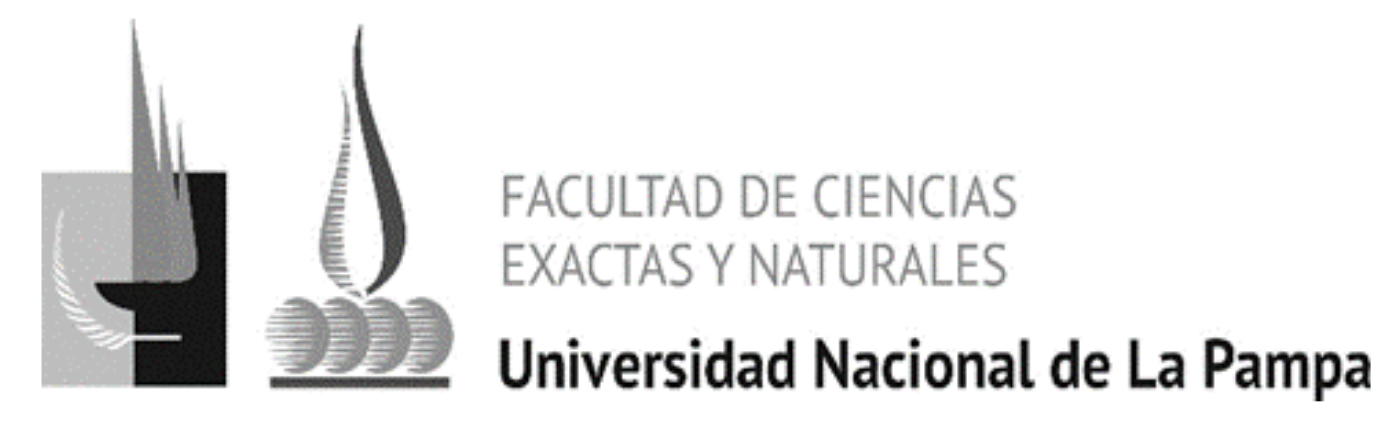
\includegraphics[scale=.3]{EscudoUNLPam.png}}]{\fancyplain{}{ 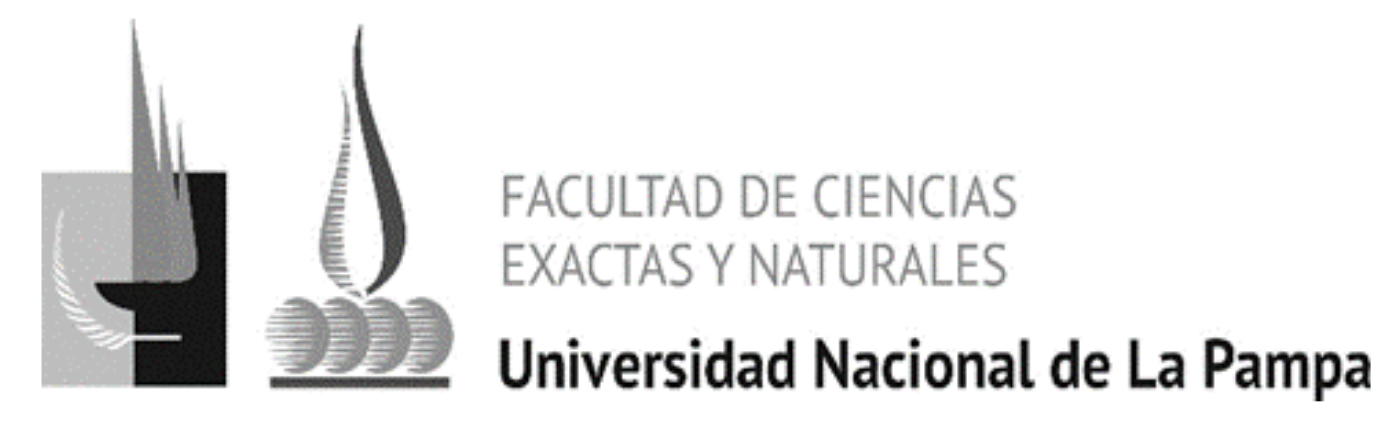
\includegraphics[scale=.3]{EscudoUNLPam.png}}}

\cfoot{}





  
  
  
  
  
  
  
\begin{document}


\hyphenation{excen-tri-ci-dad}


\begin{large}
\begin{bfseries} % \begin{scshape}
        \noindent Depto de Matem\'atica.\\
        Primer Cuatrimestre de 2022\\                                                                                                                                                                                                                                                                                                                                                
        Teoría de la Medida \\
        Práctica 3: Medida de Lebesgue

%\end{scshape}
\end{bfseries}
\end{large}
\par\noindent\rule{\textwidth}{.5pt}









\section{2019: Desde un Libro que no es Favo-Z\'o}




\begin{ejer}{} 

\textcolor{red}{Ya estaría en el teórico}
\begin{enumerate}
\item
Sean $\{I_k\}_{k=1}^n$ intervalos disjuntos.  
Probar que si $I=\bigcup\limits_{k=1}^n I_k$ entonces $l(I)=\sum\limits_{k=1}^n l(I_k)$.
\item Para cada $a,b\in \rr$, probar que $l(\{a\})=l(\{b\})$.
\item Si $I_1, I_2$ son intervalos tales que $I_1\subseteq I_2$, mostrar que $l(I_1)\leq l(I_2)$.
\item Sean $I_1,I_2,\dots,I_n$ intervalos abiertos y acotados. 
Si $I\subset \bigcup\limits_{k=1}^n I_k$, entonces $l(I)\leq \sum\limits_{k=1}^n l(I_k)$.
\end{enumerate}
\end{ejer}



\begin{ejer}{} 
\textcolor{red}{No lo pondría}
\begin{enumerate}
\item Si $I_1,I_2,\dots,I_n$ es un conjunto finito de intervalos abiertos disjuntos 2 a 2 y si 
$I$ es un intervalo abierto acotado  tal que $\bigcup\limits_{k=1}^n I_k\subset I$ entonces
$\sum\limits_{k=1}^n l(I_k) \leq l(I).$
\item Si $I_1,I_2,\dots,I_n,\dots$ es una sucesión de intervalos abiertos disjuntos 2 a 2 y si 
$I$ es un intervalo abierto acotado  tal que $\bigcup\limits_{k=1}^{\infty} I_k\subset I$ entonces
$\sum\limits_{k=1}^{\infty} l(I_k) \leq l(I).$
\end{enumerate}
\end{ejer}  

\begin{ejer}{}

\textcolor{red}{No lo pondría}
Calcular $\sum l(I_k)$ si
\begin{enumerate}
\item $I_k=\left(\frac{1}{k+1},\frac{1}{k}\right)$, para $k=1,2,\dots$ e $I=(0,1)$  con $\bigcup I_k\subset I$.
\item $I_k=\left(\frac{1}{2k},\frac{1}{2k-1}\right)$, para $k=1,2,\dots$.
\item $a_k=1+\frac{1}{2}+\dots+\frac{1}{k}-\int_1^{k+1} \frac{1}{x}\,dx $ e $I_k=(a_k,a_{k+1})$ para $k=1,2,\dots$.
\end{enumerate}
\end{ejer}  



\begin{ejer}{}\begin{enumerate}
\textcolor{red}{No lo pondría}
\item ?`Por qu\'e $\mu^*((0,1))\leq 1$?
\item ?`Es posible concluir que  $\mu^*((0,1))= 1$?
\end{enumerate}
\end{ejer}



\begin{ejer}{}  Calcular $\mu^*(A)$ si:
\begin{enumerate}
\item $A=\left\{1,\frac{1}{2},\frac{1}{3},\dots,\right\}$. \textcolor{red}{Pondría un conjunto numerable arbitrario}
\\
\underline{Ayuda:} $\frac{1}{k}\in \left(\frac{1}{k}-\frac{\epsilon}{2^k},\frac{1}{k}+\frac{\epsilon}{2^k}\right)$.
\item $A=\left\{\frac{2k-1}{2^n}:n\in\nn,\;1\leq k\leq 2^{n-1} \right\}$.
\end{enumerate}
\end{ejer}  

\begin{ejer}{} Probar que
\begin{enumerate}
\item Si $\mu^*$ fuera finitamente aditiva, entonces $\mu^*$ sería  sigma aditiva.
\item Si $\mu^*(A)=0$, entonces $\mu^*(A\cup B)=\mu^*(A)+\mu^*(B)=\mu^*(B)$.
\end{enumerate}
\end{ejer} 



\begin{ejer}{} Usando el conjunto de Vitali, probar que $\sqrt{2}$ no es equivalente a $\sqrt{3}$.
\end{ejer}

\begin{ejer}{} Mostrar que: 
\begin{enumerate}
\item $\emptyset$ y $\rr$ son conjuntos medibles Lebesgue; 
\item si $E$ es un conjunto medible Lebesgue, entonces su complemento tambi\'en lo es.
\end{enumerate}
\end{ejer} 

\begin{ejer}{} 
Mostrar que los conjuntos $ \mathcal{O}$ constituyen una $\sigma$-\'algebra.
\begin{enumerate}
\item $\mathcal{O}=\{\emptyset, \Omega\}$.
\item $\mathcal{O}$ es la colecci\'on de todos los subconjuntos de $\Omega$: $2^{\Omega}$.
\item $\Omega=\{1,2,3,\dots\}$, $\mathcal{O}=\{\emptyset,\{1,3,5,\dots,\},\{2,4,6,\dots,\},\Omega\}$.
\item $\Omega$ es cualquier conjunto no numerable y $\mathcal{O}$ es la colecci\'on de todos los subconjuntos
de $\Omega$ que son numerables o que tienen complementos numerables.
\end{enumerate}
\end{ejer} 


\begin{ejer}{} 
Si $(A_k)$ es una sucesi\'on de conjuntos en una $\sigma$-\'algebra $\mathcal{O}$, entonces
\begin{enumerate}
\item $\bigcap A_k$ pertenece a la $\sigma$-\'algebra $\mathcal{O}$.
\item $\limsup A_k=\bigcap\limits_{k\geq 1}\left(\bigcup\limits_{n\geq k} A_n\right)$ pertenece a $\mathcal{O}$.
\item $\liminf A_k=\bigcup\limits_{k\geq 1}\left(\bigcap\limits_{n\geq k} A_n\right)$ pertenece a $\mathcal{O}$.
 \end{enumerate}
 \end{ejer}  

\begin{ejer}{} 
Mostrar que el conjunto de intervalos abiertos no es una $\sigma$-\'algebra.
\\
\underline{Ayuda:} $[-1,1]=\cap \left(-1-\frac{1}{n},1+\frac{1}{n}\right)$. 
\end{ejer} 

\begin{ejer} 
Sean $\Omega$ un espacio, $\mathcal{O}_1$ y  $\mathcal{O}_2$ $\sigma$-\'algebras de subconjuntos de 
$\Omega$. \\
Probar que si $\mathcal{O}_3=\mathcal{O}_1\cap \mathcal{O}_2$, entonces $\mathcal{O}_3$ 
tambi\'en es $\sigma$-\'algebra de $\Omega$. 
\end{ejer} 


\begin{ejer}{} 
Sea $f: A\to B$ una funci\'on  y sup\'ongase que $\mathcal{B}$ es una $\sigma$-\'algebra en $B$. \\
Probar que el conjunto de im\'agenes inversas de los conjuntos en $\mathcal{B}$  forman una 
$\sigma$-\'algebra en $A$. 
\end{ejer}
 
\begin{ejer}{}
Analizar la medibilidad Lebegue de los conjuntos y calcular su medida Lebesgue cuando sea pertinente.

\begin{enumerate}
\item $E_k=\left(\frac{1}{k+1},\frac{1}{k}\right)$, $\bigcup E_k$;
\item $E_k=\left(0,1+\frac{1}{2}+\dots+\frac{1}{k}-\ln x\right)$, $\bigcap E_k$; \\
$F_k=\left(0,1+\frac{1}{2}+\dots+\frac{1}{k+1}-\ln x\right)$, $\bigcup F_k$; 
\item $E_k=\left(\frac{1+2^{\alpha}+\dots+(k-1)^{\alpha}}{k^{\alpha + 1}},1\right), \alpha>0$, $\bigcap E_k$;\\
$F_k=\left(\frac{1+2^{\alpha}+\dots+k^{\alpha}}{k^{\alpha + 1}},1\right), \alpha>0$, $\bigcup F_k$;
\item $E_k=(0,x_k)$, $x_k=(\frac{2}{1})(\frac{2}{3})(\frac{4}{3})(\frac{4}{5})\dots(\frac{2k}{2k-1})(\frac{2k}{2k+1}),$
$\bigcup E_k;$
\item N\'umeros irracionales de $(0,1)$, tiene medida positiva pero no contiene ning\'un intervalo;
\item N\'umeros de $(0,1)$ que no continen $7$ en su expresi\'on decimal.
\item Si $E$ es medible Lebesgue, $\mu(E)<\infty$ y $E\subset A$, entonces $\mu^*(A-E)=\mu^*(A)-\mu^*(E)$.
\item $\mu^*(A \cup B)+\mu^*(A\cap B) \leq \mu^*(A)+\mu^*(B)$.
\end{enumerate}
\end{ejer} 


\begin{ejer}{}
Probar que $E\subset \rr$ es medible Lebesgue si y s\'olo si existen conjuntos borelianos $B_1$
 y $B_2$ tales que $B_2\subset E\subset B_1$ y $\mu^*(B_1-B_2)=0$.
\\
\underline{Ayuda:} $B_1-B_2=(B_1-E)\cup (E-B_2)$. 
\end{ejer} 


\begin{ejer}{} 
 Sea $E$ un conjunto medible Lebesgue con $\mu(E)<\infty$.
\\Probar que existe una sucesi\'on decreciente de conjuntos abiertos $(G_k)$ tal que
$\lim \mu(G_k)=\mu (E)$.
\\
\underline{Ayuda:} $E\subset \mathcal{O}_k$ y $\mu(\mathcal{O}_k-E)<\frac{1}{k}$
y considerar 
$\mathcal{O}_1,\mathcal{O}_1\cap\mathcal{O}_2,\mathcal{O}_1\cap\mathcal{O}_2\cap\mathcal{O}_3,\dots$.
\end{ejer} 



\begin{ejer}{} 
 Sea  $E$ un conjunto medible Lebesgue con $\mu(E)<\infty$.\\
Probar que existe una sucesi\'on creciente de conjuntos cerrados $(F_k)$ tal que
$\lim \mu(F_k)=\mu (E)$.
\end{ejer} 


\section{En a\~nos anteriores desde el Fava-Z\'o}


\begin{ejer} {}
Si $I$ y $J$ son intervalos, probar que $I \cap J$ también lo es; pero que 
  no necesariamente $I \cup J$ e $I-J$ lo son. 
 \end{ejer}
  
 \begin{ejer}{}
	\begin{enumerate}
  \item Si $A$ y $B$ son conjuntos elementales disjuntos, $A \cup B$ también es 
  un conjunto elemental.
  \item Si $A$  y $B$ son conjuntos elementales, $A \cap B$ es elemental.
	\end{enumerate}
\end{ejer}
	
\begin{ejer}{}
  El disco cerrado $x^2+y^2\leq 1$ no es un conjunto $\sigma$-elemental en el plano
  $\rr^2$.
	\end{ejer}

  \begin{ejer}{} 
	La intersección de una sucesión de conjuntos $\sigma$-elementales y la diferencia 
  entre dos conjuntos $\sigma$-elementales pueden no ser $\sigma$-elementales.
 \\
  \underline{Sugerencia:} considerar el conjunto ternario de Cantor.
\end{ejer}


 \begin{ejer}{} 
	Mostrar que cualquier conjunto con medida exterior positiva contiene un conjunto 
  %acotado con medida exterior positiva. 
	\end{ejer}
 
  \begin{ejer}{} 
	Probar que si $m_e(E)>0$ y $0<\alpha<1$, entonces existe un intervalo $I$, tal que
  $m_e(E\cap I)>\alpha m(I)$.
\\
  \underline{Sugerencia:} suponiendo primero que $0<m_e(E)<\infty$, considerar un conjunto
  $\sigma$-elemental $U=\di\bigcup_{k=1}^{\infty}I_k$, tal que 
  $U\supset E$ y $m(U)<\alpha^{-1} m_e(E)$; entonces al menos uno de los intervalos $I_k$
  debe satisfacer la desigualdad del enunciado.
 \end{ejer} 

  \begin{ejer} {} 
	{\it{Decimos que un conjunto $E\subset \rr^n$ 
  {\bf{satisface la condición de Caratheodory}}
  si para cualquier conjunto $S\subset \rr^n$ se verifica}} 
  $$m_e(S\cap E)+m_e(S-E)=m_e(S). $$
%%%%%%%%%%%%%%
	\begin{enumerate}   
    \item Probar que todo conjunto medible $E$ satisface la condición de Caratheodory.
    \\
    \underline{Sugerencia:} basta probar que para cualquier conjunto $S$ se cumple
    $$m_e(S\cap E)+m_e(S-E)\leq m_e(S), $$
    en vista de que la desigualdad opuesta se cumple en cualquier caso.
 
    \item Probar que si $E_1$ y $E_2$ satisfacen la condición de Caratheodory, 
    entonces la intersección de ambos conjuntos también la satisface.
    \\
    \underline{Sugerencia:} el conjunto $S-E_1\cap E_2$ es la unión de los conjuntos 
    disjuntos $S\cap E_1-E_2$, $(S-E_1)\cap E_2$ y $(S-E_1)-E_2$.

    \item Probar que si $E$ satisface la condición de Caratheodory, entonces $E$ es medible.
    \\
    \underline{Sugerencia:} en virtud de {\it{a)}} y {\it{b)}} se puede suponer que $E$ es acotado.
	\end{enumerate}
    La moraleja del problema es que 
    %%%% 
    {\bf{``los conjuntos medibles son exactamente los que satisfacen
    la condición de Caratheodory.''}}
  \end{ejer} 
	
	
  \begin{ejer} {}
	\label{ej-guia}
  Para cualquier conjunto $E \subset \rr^n$, existe un conjunto $H$ de clase $G_{\delta}$,
  tal que $E \subset H$ y $m_e(E)=m(H)$.
	\end{ejer} 

  \begin{ejer} {}
  Si el conjunto $E$ es la unión de una sucesión creciente de conjuntos 
  $E_1\subset E_2\subset E_3\subset...$, entonces 
  $ m_e(E)=\di\lim_{k\rightarrow \infty} m_e(E_k).$
  \\
  \underline{Sugerencia:} para cada $k$ elíjase un conjunto $H_k$ de clase $G_{\delta}$,
  tal que $E_k\subset H_k$, $m(H_k)=m_e(E_k)$; los conjuntos de clase $G_{\delta}$
  $$D_k=H_k\cap H_{k+1}\cap H_{k+2}\cap... $$
  para $k=1,2,3,...$ forman una sucesión creciente que verifica $E_k \subset D_k$,
  $m(D_k)=m_e(E_k)$ y el conjunto $E$ está incluido en la unión de los $D_k$, de donde
  se sigue que $m_e(E)\leq \di\lim_{k\rightarrow \infty} m_e(E_k)$.
  \\
  La desigualdad opuesta es inmediata.
 \end{ejer}


  \begin{ejer}{}
	Probar que para cualquier  conjunto $E \subset \rr^n$ existe un conjunto $H$ de
  clase $G_{\delta}$, tal que $E \subset H$ y para cualquier conjunto medible $M$ se cumple
  $$m_e(E \cap M)=m(H\cap M).$$
 %%%%
  \underline{Sugerencia:} suponiendo primero que $m_e(E)<\infty$, considérese un conjunto
  $H$ de clase $G_{\delta}$ como en el ejercicio \ref{ej-guia}. El conjunto $M$ satisface la
  condición de Caratheodory con respecto a $E$.
   \end{ejer} 

   \begin{ejer}{}
	Probar que si $E_1$ y $E_2$ son conjuntos medibles disjuntos, entonces para cualquier
  conjunto $S \subset \rr^n$ se cumple 
  $$m_e(S\cap E_1)+m_e(S\cap E_2)=m_e(S\cap(E_1\cup E_2)). $$
  Generalizar a cualquier sucesión $(E_k)$ de conjuntos medibles disjuntos.
   \end{ejer} 

 \begin{ejer}{} 
   Si $A$ es un conjunto elemental, entonces $A$ es finitamente medible.
	\end{ejer} 
	
	 \begin{ejer}{} 
 Si $E$ y $F$ son conjuntos medibles cualesquiera, entonces
  $$m(E \cup F)+m(E \cap F)=m(E)+m(F).$$
	\end{ejer} 

   \begin{ejer}{} 
	\begin{enumerate}
  \item Sean $\{E_k\}_{k \in \nn}$ tales que $E_1 \subset E_2 \subset E_3\subset... $.
  \\
  Si $F_1=E_1$ y $F_k=E_k-E_{k-1}$ $\forall k\geq 2$, luego $\{F_k\}$ son mutuamente disjuntos
  y $$\di\bigcup_{k=1}^{\infty \atop \bullet} F_k=\bigcup_{k=1}^{\infty} E_k.$$
  \item Si $F_k=E_1-E_k$ donde $E_1\supset E_2 \supset E_3 \supset...$, entonces
  $F_1\subset F_2 \subset ...$ 
\end{enumerate} 
\end{ejer}  
%
   \begin{ejer}{}  Probar que $G \in G_{\delta}$ si y sólo si $G^c \in F_{\sigma}$.
	\end{ejer} 
  %
%
%

  \begin{ejer}{} 
	Son equivalentes:
	\begin{enumerate}
    \item $E$ es medible.
    \item $\forall \epsilon >0$ existe un conjunto cerrado $F$ tal que $F \subset E$ y $m_e(E-F)<\epsilon$.
    \item $\exists\; H \in F_{\sigma}$ tal que $H\subset E$ y $\exists\; Z$ de medida cero tal que
    $E=H\cup Z$.
	\end{enumerate}
	\end{ejer} 
%

    \begin{ejer}{} 
	Probar que para cualquier conjunto medible $E$ vale la fórmula
   $$m(E)=\sup\{m(K):K\subset E\}, $$
   donde el supremo se toma sobre todos los conjuntos compactos $K \subset E$.
\end{ejer} 

   \begin{ejer}{} 
	Sea $(E_k)$ una sucesión de conjuntos medibles. Probar que
	\begin{enumerate}
    \item $m(\liminf E_k)\leq \liminf m(E_k)$;
    \item si para alg\'un $j$, \;$m(\di\bigcup_{k\geq j}E_k)<\infty$, luego\; 
    $\limsup m(E_k)\leq m(\limsup E_k)$;
    \item si la sucesión $(E_k)$ tiende a un límite y todos los $E_k$ son subconjuntos
    de un conjunto fijo $A$ de medida finita, entonces \;$m(\lim E_k)=\lim m(E_k)$.
    \\
    Exhibir una sucesión de conjuntos $E_k$ en el intervalo unitario $[0,1]$, tal que 
    $m(\liminf E_k)<\liminf m(E_k)<\limsup m(E_k)<m(\limsup E_k)$  (todas las desigualdades estrictas).
	\end{enumerate}
	\end{ejer} 

   \begin{ejer}{} 
	Mostrar que existe un conjunto $H$ incluido en el intervalo unitario $[0,1]$, de clase
  $F_{\sigma}$, de medida uno, formado exclusivamente por puntos irracionales. 
  \\
  Mostrar que $H$ es unión numerable de conjuntos cerrados con interior vacío.
\end{ejer} 

   \begin{ejer}{} 
	Demostrar que $\Sigma$ es $\sigma$-álgebra si:
	\begin{enumerate}
    \item $\Sigma=\{Z:m(Z)=0 \;\;\text{ó}\;\; m(Z^c)=0\}$;
    \item $\Sigma=\mathcal{P}(X)$.
	\end{enumerate}
	\end{ejer} 

   \begin{ejer}{} 
	Si $\Sigma$ es $\sigma$-álgebra y $E_i \in  \Sigma$ para $i=1,2,...$; entonces\;
  $\di\bigcap_{i=1}^{\infty} E_i \in \Sigma$.
	\end{ejer} 

   \begin{ejer}{} 
	Si $I$ es un intervalo, luego $T_z(I)$ también lo es.
	\end{ejer} 
  
   \begin{ejer}{} 
	?`Cómo son los subconjuntos medibles del conjunto de Vitali?
\end{ejer} 


\end{document}
